\documentclass[pdf,randalg,slideColor,colorBG]{prosper}

\usepackage[latin1]{inputenc}
%\usepackage[portuguese]{babel}
\usepackage[english]{babel}
 \title{Census of Prime Spaces with a Small Blink Presentation}
 \author{Lauro Didier Lins}
 \email{lauro.lins@gmail.com}
 \institution{
 UFPE - Brasil \\
 September 29, 2006
 }

% Optional: text to put in the bottom of each slide.
% By default, the title of the talk will be placed there.
\slideCaption{\textit{Lauro Lins, UFPE}}

\ptsize{8}

%----------------------------------------------------------------- COMMANDS

\newcommand{\VerticalGap}[1]{\rule[#1]{0cm}{0cm}}
\newcommand{\HorizontalGap}[1]{\rule[0cm]{#1}{0cm}}
\newcommand{\Real}{\text{\bf R}}

%\newcommand{\AoverB}[2]{\begin{tabular}{c} {#1} \\[-2pt] {#2} \end{tabular}}
\newcommand{\Vspace}[1]{\rule[#1]{0cm}{0cm}}
\newcommand{\AoverB}[2]{\vbox{\hbox{#1}\hbox{\Vspace{0.2cm}#2}}}
\newcommand{\problem}[2]{

\begin{center}
   \fbox{
      \begin{minipage}{#1}
      #2
      \end{minipage}}
\end{center}}

\newcommand{\Space}{\hspace{0.2cm}}
\newcommand{\prova}[1]{
\begin{small}
{\it Prova} \Space #1 \hfill $\square$
\end{small}}

\newcommand{\proposicao}[2]{
{\large \bf Prop. #1} \Space #2}

\newcommand{\definicao}[2]{
{\large \bf Def. #1} \Space #2}

%------------------------------------------------------------------------ DOCUMENT

\begin{document}
\maketitle
%------------------------------------------------------------------------ SLIDE


%%% Slide 1

\overlays{3}{
\begin{slide}{Spaces}
\begin{itemstep}
\item Topology deals with, among other objects, the so
called {\em 3-manifolds}. A basic type of 3-manifolds is a {\em
closed, connected, oriented 3-manifold}.

\bigskip

\item {{\bf Definition:}

\medskip

\begin{center} {\large
In this work, the term {\em space} is a synonym of a {\em closed,
connected, oriented 3-manifold}.}
\end{center}}

\bigskip

\item{{\bf Examples of Spaces:}
\begin{center} {\large
$S^3$, $S^1\!\times\!S^2$, $L_{2,1}$, $L_{3,1}$} \end{center}}


\end{itemstep}
\end{slide}}


%%% Slide 2

\overlays{3}{
\begin{slide}{Blinks}
\begin{itemstep}

\item {
In 1994, Lins and Kauffman \cite{KauffmanLins1994} introduced a new
way to present spaces. They named their new presentation as {\em
blinks}. In fact, on their work, blinks were appreciated by being a
new concise presentation for spaces, but its main importance there
was its use as an intermediate step to convert a {\em blackboard
framed link} presentation of a space into a {\em 3-gem} presentation
of the same space. }

\smallskip

\item {{\bf Definition:}

\begin{center} {\large A {\em blink} is a plane graph with each edge being either
{\em red} or {\em green}}.\end{center}

   \begin{center}
      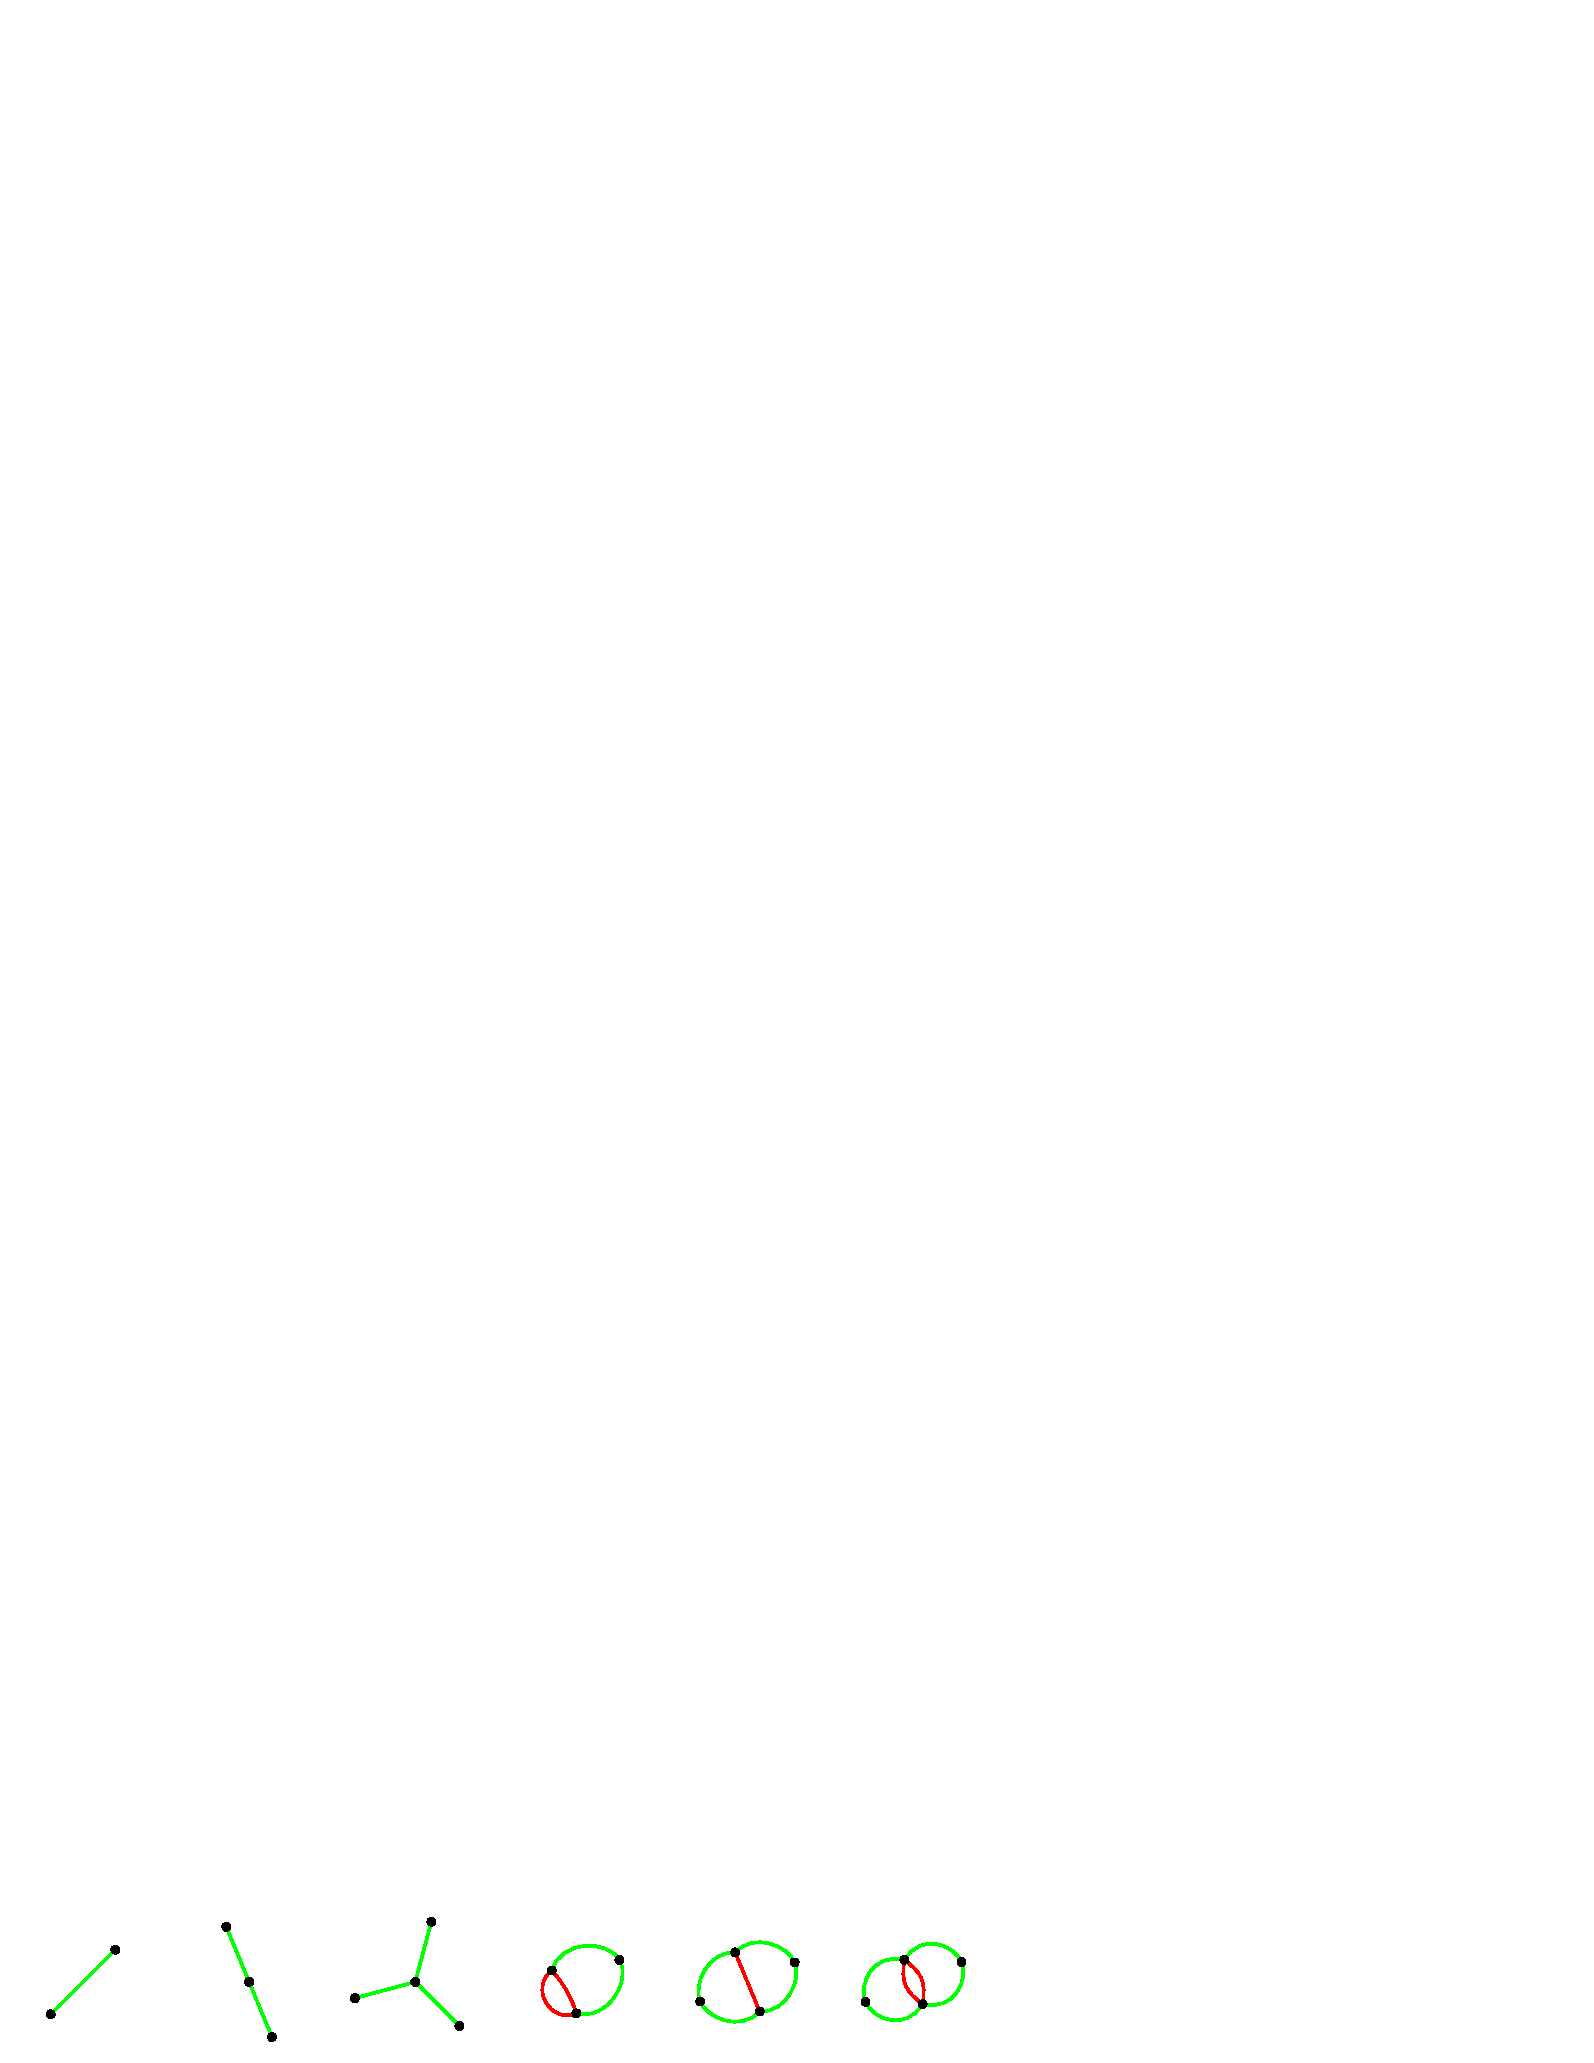
\includegraphics[width=10cm]{fig/blinkExamples.eps}
   \end{center}
   The {\em size of a blink} is its number of edges.}


\item {{\bf Theorem:}

\begin{center} {\large Any space can be presented by a
blink (in fact, infinitely many blinks) and any blink induces a
space}.
\end{center}}

\end{itemstep}

\end{slide}}

%%% Slide 3

\overlays{4}{
\begin{slide}{Blinks}
\begin{itemstep}

\item {The idea that blinks were an elegant space presentation, with a
cleaner aspect than other space presentations ({\it e.g.} blackboard
framed links, special spines, heegaard diagrams) allied to the fact
that they were not directly explored before were the initial
motivation for this work.}

\bigskip

\item {So, the main idea was:
\medskip

\centerline{\large Explore blinks as a space presentation.} }

\smallskip


\smallskip

\item {Some interesting questions:}

\smallskip

\begin{center}(1) What spaces have a ``small'' blink
presentation? For instance, with less than 9 edges? ({\it i.e.} size
$\leq 9$?)\end{center}

\begin{center}(2) Let $\alpha$ be the minimum size of any blink that
induces space $S$. Is $\alpha$ an important number for $S$? Does
this number have analogues in other forms of viewing spaces?
\end{center}

\begin{center}(3) Blinks, as a connection of spaces with plane
graphs, permits questions like: what are the spaces of 3-connected
blinks?
\end{center}

\begin{center}(4) Is there a ``blink calculus'' that connects two blinks
if and only if they induce the same space?
\end{center}

\end{itemstep}

\end{slide}}

\begin{slide}{References}

\bibliographystyle{alpha}
\begin{thebibliography}{100}

\bibitem[KL94]{KauffmanLins1994}
Louis~H. Kauffman and Sostenes Lins.
\newblock {\em Temperley-Lieb Recoupling Theory and Invariants of 3-Manifolds
  (AM-134)}.
\newblock Princeton University Press, 1994.
\end{thebibliography}

\end{slide}




\end{document}
